\documentclass{beamer}

\pdfmapfile{+sansmathaccent.map}


\mode<presentation>
{
  \usetheme{Warsaw} % or try Darmstadt, Madrid, Warsaw, Rochester, CambridgeUS, ...
  \usecolortheme{seahorse} % or try seahorse, beaver, crane, wolverine, ...
  \usefonttheme{serif}  % or try serif, structurebold, ...
  \setbeamertemplate{navigation symbols}{}
  \setbeamertemplate{caption}[numbered]
} 


%%%%%%%%%%%%%%%%%%%%%%%%%%%%
% itemize settings

\definecolor{mypink}{RGB}{255, 30, 80}
\definecolor{mydarkblue}{RGB}{60, 160, 255}
\definecolor{myblackblue}{RGB}{40, 40, 120}
\definecolor{myblue}{RGB}{240, 240, 255}
\definecolor{mygreen}{RGB}{0, 200, 0}
\definecolor{mygreen2}{RGB}{205, 255, 200}
\definecolor{mygray}{gray}{0.8}
% \definecolor{mydarkgray}{gray}{0.4}
\definecolor{mydarkgray}{RGB}{80, 80, 160}

\setbeamertemplate{itemize items}[default]

\setbeamertemplate{itemize item}{\color{myblackblue}$\blacksquare$}
\setbeamertemplate{itemize subitem}{\color{mydarkblue}$\blacktriangleright$}
\setbeamertemplate{itemize subsubitem}{\color{mygray}$\blacksquare$}

\setbeamercolor{palette quaternary}{fg=white,bg=mydarkgray}
\setbeamercolor{titlelike}{parent=palette quaternary}

\setbeamercolor{palette quaternary2}{fg=black,bg=myblue}
\setbeamercolor{frametitle}{parent=palette quaternary2}

\setbeamerfont{frametitle}{size=\Large,series=\scshape}
\setbeamerfont{framesubtitle}{size=\normalsize,series=\upshape}





%%%%%%%%%%%%%%%%%%%%%%%%%%%%
% block settings

\setbeamercolor{block title}{bg=red!30,fg=black}

\setbeamercolor*{block title example}{bg=mygreen!40!white,fg=black}

\setbeamercolor*{block body example}{fg= black, bg= mygreen2}


%%%%%%%%%%%%%%%%%%%%%%%%%%%%
% URL settings
\hypersetup{
    colorlinks=true,
    linkcolor=blue,
    filecolor=blue,      
    urlcolor=blue,
}

%%%%%%%%%%%%%%%%%%%%%%%%%%

\renewcommand{\familydefault}{\rmdefault}

\usepackage{amsmath}
\usepackage{mathtools}

\usepackage{subcaption}

\usepackage{qrcode}

\DeclareMathOperator*{\argmin}{arg\,min}
\newcommand{\bo}[1] {\mathbf{#1}}

\newcommand{\dx}[1] {\dot{\mathbf{#1}}}
\newcommand{\ma}[4] {\begin{bmatrix}
    #1 & #2 \\ #3 & #4
    \end{bmatrix}}
\newcommand{\myvec}[2] {\begin{bmatrix}
    #1 \\ #2
    \end{bmatrix}}
\newcommand{\myvecT}[2] {\begin{bmatrix}
    #1 & #2
    \end{bmatrix}}
    
    

\newcommand{\mydate}{Spring 2022}
\newcommand{\mygit}{\textcolor{blue}{\href{https://github.com/SergeiSa/Control-Theory-Slides-Spring-2022}{github.com/SergeiSa/Control-Theory-Slides-Spring-2022}}}


\newcommand{\bref}[2] {\textcolor{blue}{\href{#1}{#2}}}




%%%%%%%%%%%%%%%%%%%%%%%%%%%%
% code settings

\usepackage{listings}
\usepackage{color}
% \definecolor{mygreen}{rgb}{0,0.6,0}
% \definecolor{mygray}{rgb}{0.5,0.5,0.5}
\definecolor{mymauve}{rgb}{0.58,0,0.82}
\lstset{ 
  backgroundcolor=\color{white},   % choose the background color; you must add \usepackage{color} or \usepackage{xcolor}; should come as last argument
  basicstyle=\footnotesize,        % the size of the fonts that are used for the code
  breakatwhitespace=false,         % sets if automatic breaks should only happen at whitespace
  breaklines=true,                 % sets automatic line breaking
  captionpos=b,                    % sets the caption-position to bottom
  commentstyle=\color{mygreen},    % comment style
  deletekeywords={...},            % if you want to delete keywords from the given language
  escapeinside={\%*}{*)},          % if you want to add LaTeX within your code
  extendedchars=true,              % lets you use non-ASCII characters; for 8-bits encodings only, does not work with UTF-8
  firstnumber=0000,                % start line enumeration with line 0000
  frame=single,	                   % adds a frame around the code
  keepspaces=true,                 % keeps spaces in text, useful for keeping indentation of code (possibly needs columns=flexible)
  keywordstyle=\color{blue},       % keyword style
  language=Octave,                 % the language of the code
  morekeywords={*,...},            % if you want to add more keywords to the set
  numbers=left,                    % where to put the line-numbers; possible values are (none, left, right)
  numbersep=5pt,                   % how far the line-numbers are from the code
  numberstyle=\tiny\color{mygray}, % the style that is used for the line-numbers
  rulecolor=\color{black},         % if not set, the frame-color may be changed on line-breaks within not-black text (e.g. comments (green here))
  showspaces=false,                % show spaces everywhere adding particular underscores; it overrides 'showstringspaces'
  showstringspaces=false,          % underline spaces within strings only
  showtabs=false,                  % show tabs within strings adding particular underscores
  stepnumber=2,                    % the step between two line-numbers. If it's 1, each line will be numbered
  stringstyle=\color{mymauve},     % string literal style
  tabsize=2,	                   % sets default tabsize to 2 spaces
  title=\lstname                   % show the filename of files included with \lstinputlisting; also try caption instead of title
}


%%%%%%%%%%%%%%%%%%%%%%%%%%%%
% URL settings
\hypersetup{
    colorlinks=false,
    linkcolor=blue,
    filecolor=blue,      
    urlcolor=blue,
}

%%%%%%%%%%%%%%%%%%%%%%%%%%

%%%%%%%%%%%%%%%%%%%%%%%%%%%%
% tikz settings

\usepackage{tikz}
\tikzset{every picture/.style={line width=0.75pt}}


\title{Verification of the simulation results}
\subtitle{Math and modeling for high school}
\author{by Sergei Savin}
\centering
\date{Fall 2022}



\begin{document}
\maketitle


\begin{frame}{Analytic verification}
	% \framesubtitle{Part 1}
	\begin{flushleft}
		
		Consider a simple differential equation, where $y(0) = 1$:
		
		\begin{equation}
			\dot y = -10t - 3
		\end{equation}
	
		Its solution is $y = -5t^2-3t+1$. We can \emph{verify} it by taking a derivative:
		
		\begin{equation}
			\frac{d}{dt}(-5t^2-3t+1) = -10t-3 \ \ \qed
		\end{equation}		
		
	\end{flushleft}
\end{frame}




\begin{frame}{General case}
	% \framesubtitle{Part 1}
	\begin{flushleft}
		
		In a general case, as long as the equation is represented in the form:
		
		\begin{equation}
			g(y, \dot y, t) = 0
		\end{equation}		
	%
	and the solution is given as $y = y(t)$, we can find derivative of the solution and and check whether or not it satisfies the equation.
		
	\end{flushleft}
\end{frame}





\begin{frame}{Numerical solutions}
	% \framesubtitle{Part 1}
	\begin{flushleft}
		
		But what do we do if we only have a numerical solution, a table of numbers that approximate $y = y(y)$, a solution to a differential equation?
		
		\bigskip
		
		One option is to approximate the derivative of that solution, and repeat the process as before. But here we risk getting into numerical issues - how do we know that the errors are not due to approximating derivatives, rather than approximating the solution?
		
		\bigskip
		
		Another approach is to use our knowledge of the problem to verify the solution.
		
	\end{flushleft}
\end{frame}




\begin{frame}{Conservation laws}
	% \framesubtitle{Part 1}
	\begin{flushleft}
		
		One of the sources of important knowledge for the physical problems are the conservation laws. If some quantity has to be conserved, a solution should obey this principle. When it does not, or when it deviates - we see a sign of numerical errors.
		
		\bigskip
		
		For example, a satellite with only gravity acting on it will conserve its total energy - gravity is a conservative force. 
		
	\end{flushleft}
\end{frame}



\begin{frame}{Potential energy of a satellite}
%\framesubtitle{Gravity model}
	\begin{flushleft}
		
	Remember the model of gravitational force:
		
		\begin{equation}
			f = G \frac{m M}{h^2}
		\end{equation}
	
		where $f$ is the magnitude of the gravitational force, $m$ is the mass of the satellite, $M$ is the mass of the Earth and $h$ is the distance between the center of the Earth and the satellite.
	
		\bigskip
	
		Potential energy associated with the position of a mass in a gravitational field is:
		
		\begin{equation}
			P = -G \frac{m M}{h}
		\end{equation}
		
		
	\end{flushleft}
\end{frame}



\begin{frame}{Potential energy of a satellite}
	\begin{flushleft}
		
		Same as the gravity force can be re-written to include vector-valued position:
		
		\begin{equation}
			\bo{f} = -G \frac{m M}{||\bo{r}||^3} \bo{r}
		\end{equation}		 	 
	
	...the potential energy can be re-written the same way:
	
	\begin{equation}
		P = -G \frac{m M}{||\bo{r}||}
	\end{equation}
	
	The simplicity has to do with the fact that potential energy is a scalar, it does not have a direction, unlike the force of gravity.
		
	\end{flushleft}
\end{frame}


\begin{frame}{Kinetic energy of a satellite}
	\begin{flushleft}
		
		The kinetic energy of a satellite is much simpler to define. Let us remember the kinetic energy of a point mass:
		
		\begin{equation}
			K = \frac{1}{2} m v^2
		\end{equation}
	%
	where $v$ - velocity of the mass. For a satellite, the only thing different is that the velocity is a vector, so a square is replaced with a dot product with itself:
	
			\begin{equation}
		K = \frac{1}{2} m \dot{\bo{r}}\T \dot{\bo{r}}
			\end{equation}
	
		
	\end{flushleft}
\end{frame}




\begin{frame}{Total energy of a satellite}
	\begin{flushleft}
		
		Since there are no non-conservative forces acting on the satellite, the total energy of the satellite will be conserved:
		
			
		\begin{equation}
			E = P + K = const
		\end{equation}
			
		\begin{equation}
			-G \frac{m M}{||\bo{r}||} +  \frac{1}{2} m \dot{\bo{r}}\T \dot{\bo{r}} = const
		\end{equation}
	
		This does not depend on mass of the satellite:
		
		\begin{equation}
			-G \frac{M}{||\bo{r}||} +  \frac{1}{2} \dot{\bo{r}}\T \dot{\bo{r}} = const
		\end{equation}		
		
	\end{flushleft}
\end{frame}



\begin{frame}{Total energy of a satellite}
	\begin{flushleft}
		
		Here we illustrate a solution for a satellite orbit, taking into account earth rotation. Not how small the error interns of the change of total energy is (0.5 J):
		
		% TODO: \usepackage{graphicx} required
		\begin{figure}
			\centering
			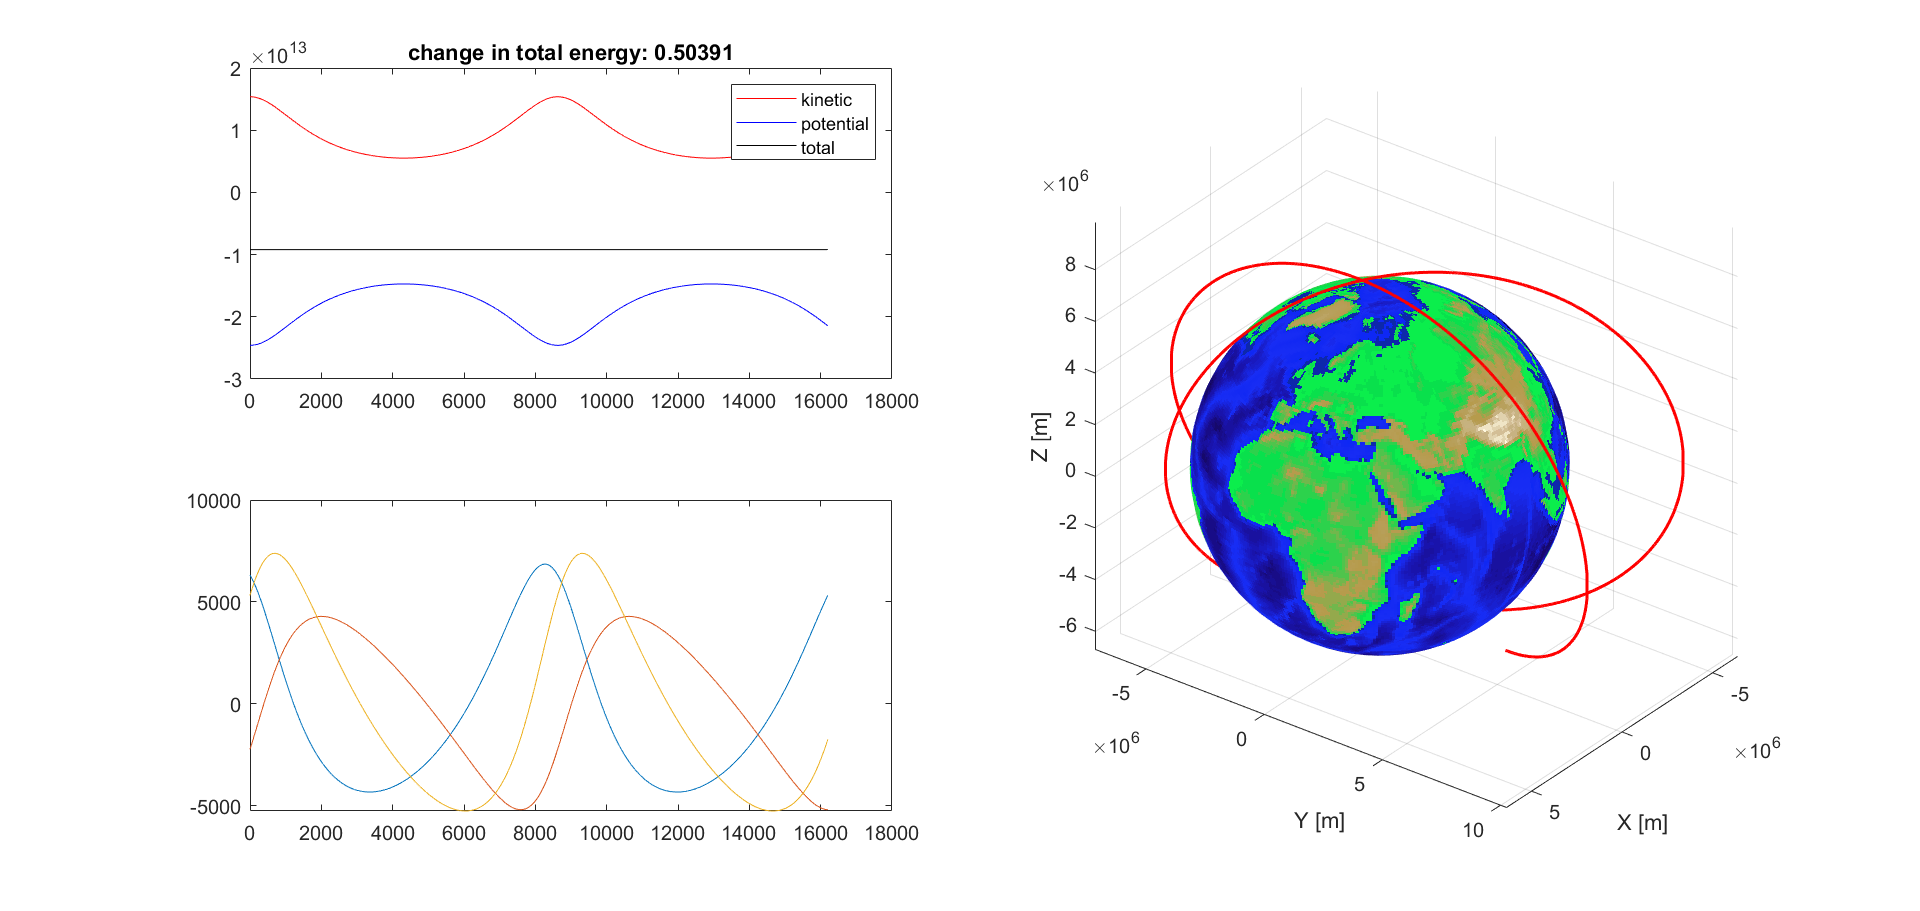
\includegraphics[width=0.7\linewidth]{Energy}
			\caption{(high-accuracy settings) total energy study for an elliptical orbit; the graph in the left top corner is the energy (red is kinetic, blue is the potential, black is total), left bottom is the velocity graphs}
			\label{fig:energy}
		\end{figure}
		
		
	\end{flushleft}
\end{frame}




\begin{frame}{Total energy of a satellite}
	\begin{flushleft}
		
		If we decrease the accuracy settings, we get a completely different picture. The error now is $-1.7 \cdot 10^{11}$:
		
		% TODO: \usepackage{graphicx} required
		\begin{figure}
			\centering
			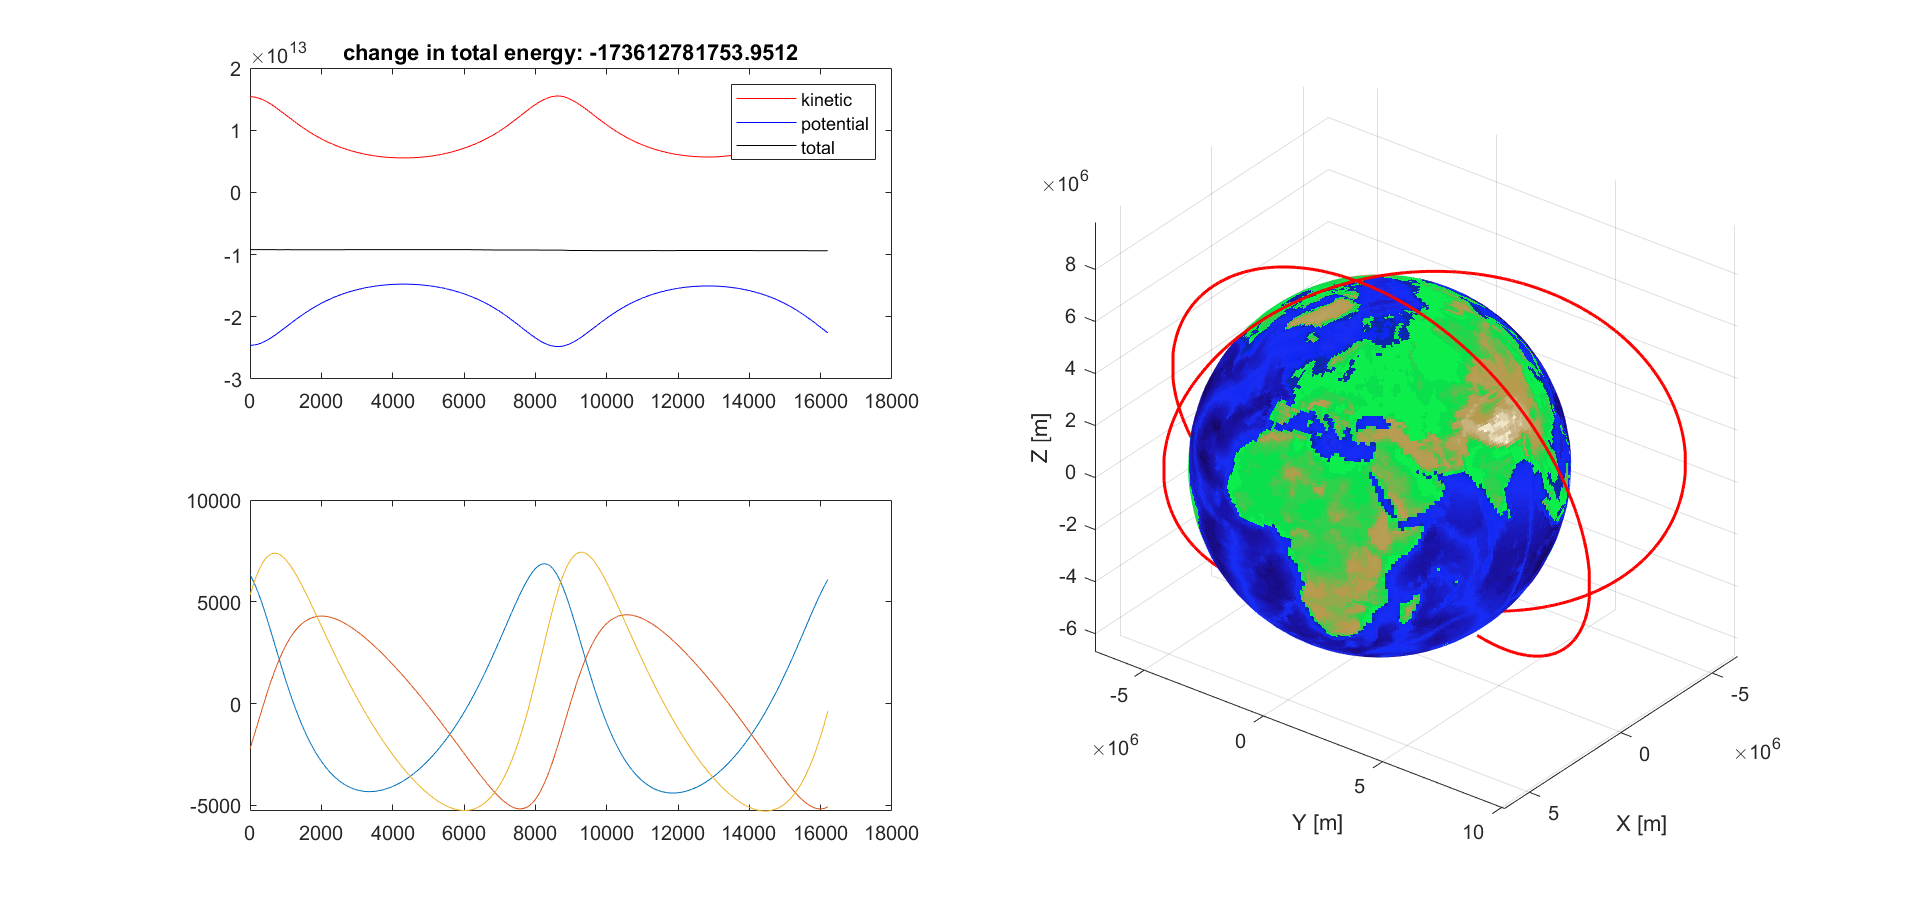
\includegraphics[width=0.7\linewidth]{Energy_high_error}
			\caption{(low-accuracy settings) total energy study for an elliptical orbit; the graph in the left top corner is the energy (red is kinetic, blue is the potential, black is total), left bottom is the velocity graphs}
			\label{fig:energy}
		\end{figure}
		
		
	\end{flushleft}
\end{frame}



\begin{frame}{Limits of the total energy verification}
	% \framesubtitle{Part 1}
	\begin{flushleft}
		
		The conservation of total energy only works when there is no external forces performing force. For example:
		
		\begin{itemize}
			\item It works for planets, passive satellites, particles;
			
			\item It does not work for rockets and spaceship (during burn), airplanes, vehicles and robots.
		\end{itemize}
		
	\end{flushleft}
\end{frame}



\begin{frame}{Other verification options}
	% \framesubtitle{Part 1}
	\begin{flushleft}
		
		It is not just total energy; we use other conserved quantities (angular momentum, etc.) or constraints:
		
		\begin{itemize}
	\item If an impact model si given, we can check the energy before and after impact;
	
	\item If a body contacts something (rolling down a surface) we can check if it penetrates the surface or stays on top of it.
	
	\item If an external force acts on a body, we can check that the total change in energy corresponds to the work performed by that body.
		\end{itemize}		
		
	\end{flushleft}
\end{frame}




\begin{frame}{Project}
	% \framesubtitle{Part 1}
	\begin{flushleft}
		
		\centerline{Now - to your individual projects!}
		
	\end{flushleft}
\end{frame}


\begin{frame}{Project}
	% \framesubtitle{Part 1}
	\begin{flushleft}
		
		\begin{block}{Project}
			Simulate a trajectory of a satellite from a given point (in West-North coordinates), and a given altitude, such that the trajectory (circular) goes over the North Pole:
			
			\begin{itemize}
				\item Draw the trajectory.
				
				\item Show which change in direction of the velocity can lead to the orbit becoming elliptical. Show how the increase in the velocity changes the shape of the trajectory.
				
				\item Implement a check on the satellite entering the Earth atmosphere.
				
				\item Implement a check on satellite leaving the Earth orbit.
				
				\item Implement a check on total energy.
				
			\end{itemize}
		\end{block}
	%
	We will grade technical soundness, originality and visual aspect of the solution.
		
	\end{flushleft}
\end{frame}


\begin{frame}{Thank you!}
\centerline{Lecture slides are available via Moodle.}
\bigskip
\centerline{You can help improve these slides at:}
\centerline{\mygit}
\bigskip
\centerline{Check Moodle for additional links, videos, textbook suggestions.}
\bigskip

\centerline{\textcolor{black}{\qrcode[height=1.6in]{https://github.com/SergeiSa/Extra-math-for-high-school}}}

\end{frame}

\end{document}
